%-------------------------------------------------------------------------
\section{Introduction}
\label{sec:intro}

The proliferation of egocentric video content, particularly in instructional domains such as cooking, has created unprecedented opportunities for developing intelligent assistive systems. These systems can help users learn new skills, identify mistakes in real-time, and provide personalized guidance. However, detecting procedural errors in such videos remains a challenging task that requires understanding both visual observations and their semantic relationship to the underlying procedural knowledge encoded in textual instructions.

\begin{figure}[t]
  \centering
  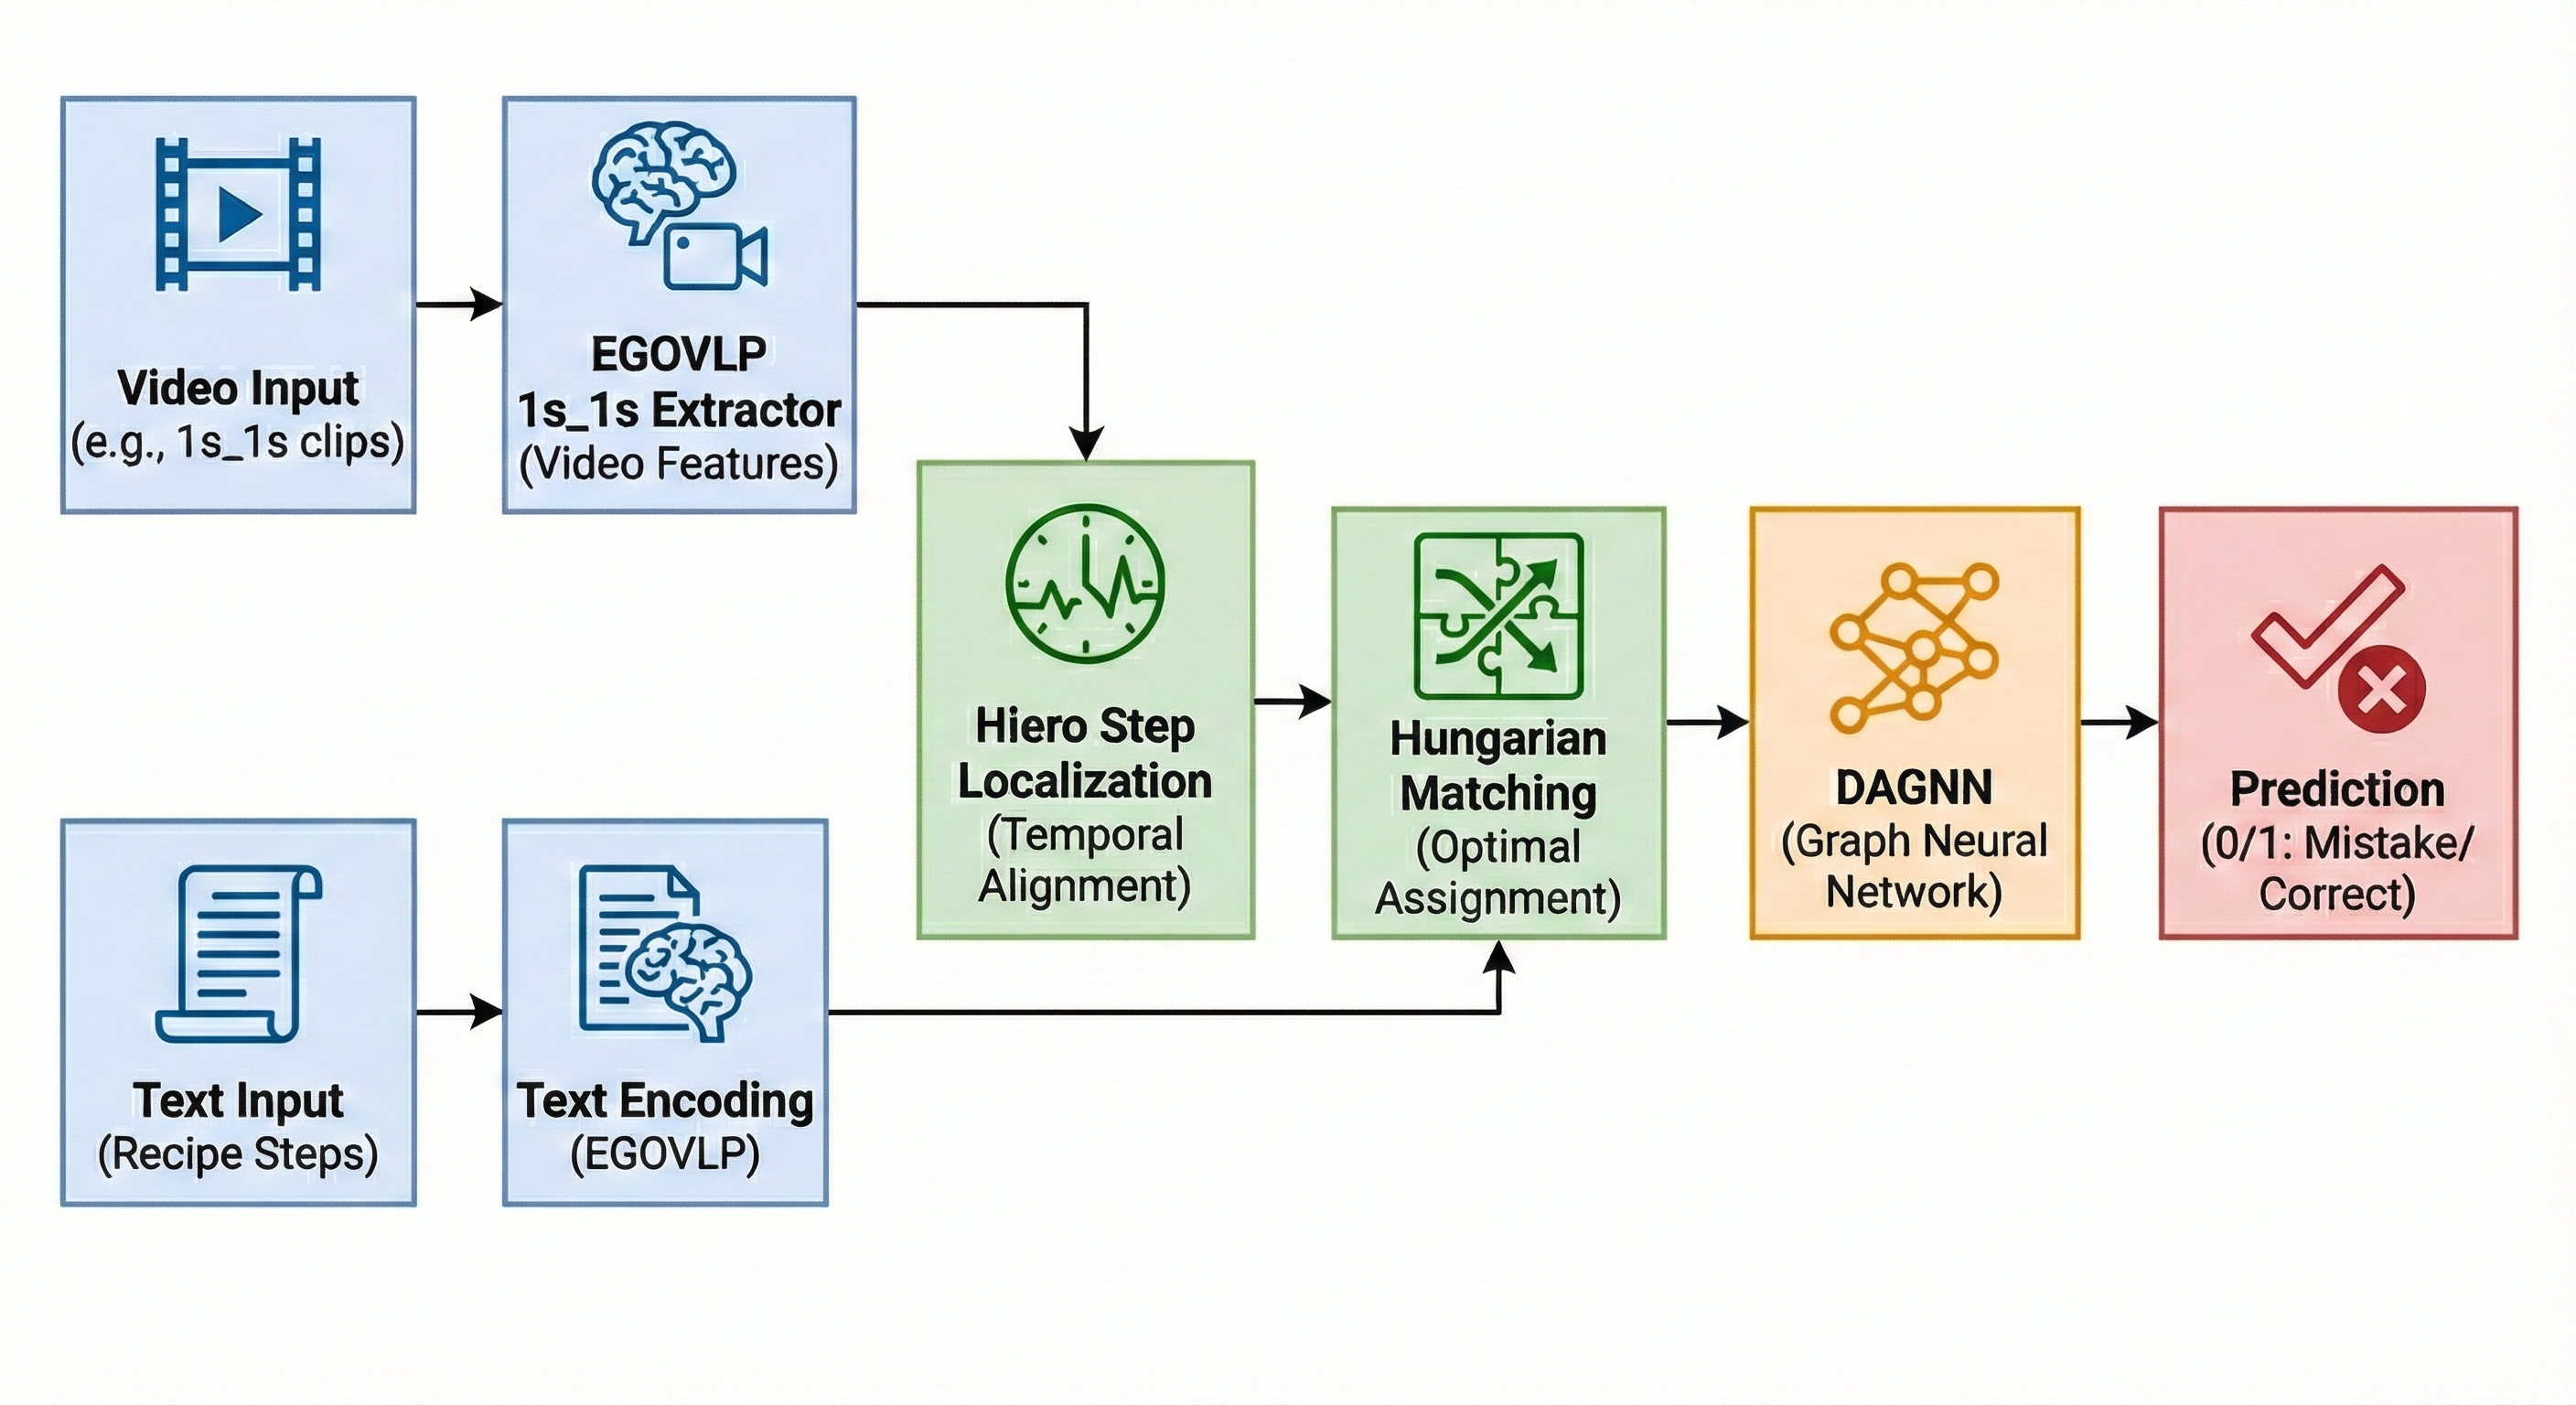
\includegraphics[width=\columnwidth]{figures/figure_1.png}
  \caption{Overview of our procedural error detection framework. We model cooking recipes as directed acyclic graphs and align visual observations from egocentric videos with textual recipe steps using multimodal embeddings.}
  \label{fig:overview}
\end{figure}

Cooking is a particularly suitable domain for studying procedural error detection due to its rich structure: recipes naturally form directed acyclic graphs (DAGs) where steps must be executed in a specific causal order, and deviations from this order or execution errors can significantly impact the final outcome. Moreover, egocentric cooking videos capture the natural first-person perspective of task execution, making them highly relevant for real-world applications in augmented reality, assistive robotics, and personalized education systems.

Despite recent advances in video understanding and multimodal learning, procedural error detection faces several fundamental challenges. First, there exists a significant \textbf{semantic gap} between low-level visual features extracted from videos and high-level procedural concepts described in recipe instructions. Second, the \textbf{temporal alignment problem} requires establishing correspondences between variable-length sequences of observed actions and prescribed recipe steps, which may not be in perfect temporal alignment. Third, the \textbf{causal structure} of recipes introduces dependencies that must be respected: an action can only be identified as erroneous when considering its context within the broader procedural graph.

Traditional approaches to action recognition focus on classifying isolated actions without considering their procedural context or relationships to textual instructions. While recent work on egocentric video understanding has made progress in action segmentation and step localization, these methods typically operate in isolation without explicitly modeling the structured knowledge inherent in procedural tasks.

In this work, we propose a novel approach that explicitly addresses these challenges by formulating procedural error detection as a graph-based multimodal learning problem. Our method leverages \textbf{Directed Acyclic Graph Neural Networks (DAGNNs)} to model the causal structure of cooking recipes while integrating visual and textual information at the node level. Specifically, we use EgoVLP visual embeddings extracted from video segments and recipe text embeddings, aligned through the Hungarian algorithm to establish semantic correspondences between observed actions and recipe steps. The resulting multimodal graph representation preserves both the procedural structure and the semantic alignments, enabling the model to reason about errors in context.

Our approach introduces several key technical contributions. We design a learnable projection layer that maps high-dimensional concatenated embeddings (1536-dimensional) to a more compact space (256-dimensional) suitable for graph convolution operations. We employ the Hungarian algorithm for optimal bipartite matching between visual observations and recipe steps based on cosine similarity in the embedding space. We explicitly handle unmatched nodes by encoding them with zero visual features, allowing the model to distinguish between observed and unobserved steps.

We evaluate our approach on the Captain Cook 4D dataset~\cite{captaincook4d}, a challenging benchmark for egocentric cooking video understanding. Our experiments reveal important insights about the difficulty of this task: despite the theoretical soundness of our approach, we observe that our model achieves performance below a simple dummy baseline system. Through careful analysis, we identify two primary factors contributing to these results: (\textit{i}) the \textbf{limited dataset size}, which provides insufficient training examples for learning robust multimodal representations, and (\textit{ii}) the \textbf{limitations of zero-shot unsupervised step localization} using the HiERO model, which introduces noise in the visual embeddings and misalignments in the Hungarian matching process.

These negative results, while disappointing, provide valuable lessons for the research community. They highlight the \textbf{critical importance of high-quality step localization} as a prerequisite for procedural error detection, suggest that \textbf{supervised approaches with larger annotated datasets} are necessary for this challenging task, and demonstrate that the \textbf{semantic gap between vision and language} in procedural domains remains a significant open problem that requires further investigation.

The main contributions of this paper are:
\begin{enumerate}
    \item A novel graph-based framework for procedural error detection that explicitly models the causal structure of cooking recipes using DAGNNs while integrating multimodal visual and textual information.
    \item A systematic approach for aligning visual observations with recipe steps using Hungarian matching on learned embedding spaces, with explicit handling of unmatched procedural steps.
    \item An extensive empirical analysis on the Captain Cook 4D dataset that reveals the limitations of zero-shot unsupervised approaches and provides insights into the requirements for successful procedural error detection.
    \item A transparent discussion of negative results that identifies dataset size and step localization quality as critical bottlenecks, providing valuable guidance for future research in this domain.
\end{enumerate}
